% ----------------------------------------------------------------------------
%                             Proposta de Desenvolvimento
% ----------------------------------------------------------------------------
\chapter{Proposta}
\label{chap:proposta}

\vspace{0.2cm}
\section{Cronograma}

O Quadro 1 apresenta o cronograma do trabalho, que ilustra as etapas fundamentais do desenvolvimento e da pesquisa distribuídas ao longo dos dois semestres letivos de 2026. Cada etapa planeada visa garantir a realização estruturada e eficiente das atividades, culminando na conclusão e defesa do trabalho final.

\vspace{0.2cm}
\noindent O planeamento está dividido em quatro fases principais:

\begin{enumerate}
    \item \textbf{Fase de Estruturação e Fundamentação (Fev/26 a Abr/26):} Inclui a definição do tema, delimitação do problema e o levantamento bibliográfico sobre TDAH e TOD. Nesta fase também foi realizado o levantamento de requisitos com os educadores para subsidiar a construção do sistema.

    \item \textbf{Fase de Design e Prototipação (Abr/26 a Jun/26):} Abrange o planeamento visual da solução em formato Web Responsivo, com foco na criação dos ecrãs no Figma para definir a Interface de Utilizador (UI/UX). Esta etapa contempla a redação do Pré-TCC e a sua apresentação.

    \item \textbf{Fase de Desenvolvimento e Validação (Ago/26 a Out/26):} Envolve a implementação do sistema em código (React.js), a configuração da base de dados em nuvem (Firebase) e a realização de testes de usabilidade e funcionamento do software.

    \item \textbf{Fase de Finalização e Entrega (Out/26 a Dez/26):} Foca-se nos ajustes finais do sistema após a fase de testes. Esta etapa inclui a redação final do TCC, a formatação nas normas ABNT e culmina com a Apresentação e Defesa Final do Trabalho.
\end{enumerate}

\begin{table}[H]
\centering
\caption{Cronograma de atividades do TCC (2026)}
\label{quadro:cronograma}
\renewcommand{\arraystretch}{1.3} 
\setlength{\tabcolsep}{4pt} 
\small 
\begin{tabular}{|p{4.5cm}|c|c|c|c|c|c|c|c|c|c|}
\hline

\multicolumn{1}{|c|}{\textbf{Etapas do Projeto}} & \multicolumn{10}{c|}{\textbf{Período (Mês)}} \\ \cline{2-11} 
 & \textbf{fev} & \textbf{mar} & \textbf{abr} & \textbf{mai} & \textbf{jun} & \textbf{ago} & \textbf{set} & \textbf{out} & \textbf{nov} & \textbf{dez} \\ \hline

Escolha do tema e delimitação do problema & X & & & & & & & & & \\ \hline
Levantamento bibliográfico e sistemas similares & X & X & & & & & & & & \\ \hline
Levantamento e análise de requisitos & & X & X & & & & & & & \\ \hline
Planeamento e prototipação das telas no Figma & & & X & X & & & & & & \\ \hline
Redação parcial do TCC (Metodologia e Cap. Iniciais) & & & X & X & & & & & & \\ \hline
Revisão com o orientador e formatação & X & X & X & X & X & X & X & X & X & X \\ \hline
Apresentação do Pré-TCC & & & & & X & & & & & \\ \hline
Configuração da Base de Dados (Firebase) & & & & & & X & & & & \\ \hline
Implementação do sistema web responsivo (React) & & & & & & X & X & X & & \\ \hline
Testes de funcionalidade e ajustes & & & & & & & & X & X & \\ \hline
Redação final do TCC (Resultados e Conclusão) & & & & & & & & X & X & \\ \hline
Revisão final, preparação e ensaio da apresentação & & & & & & & & & X & \\ \hline
Apresentação final do TCC & & & & & & & & & & X \\ \hline
\end{tabular}

\vspace{0.2cm}
\legend{Fonte: Elaborado pelo autor (2026)}
\end{table}

\section{Requisitos de Usuário (RU)}

Os requisitos de usuário foram elaborados visando o acompanhamento adequado dos alunos com TDAH e TOD, levando em conta o suporte oferecido por professores e responsáveis durante a utilização da plataforma web.

\vspace{0.3cm}
RU01 - Organização das Salas: Como educador, eu preciso criar e estruturar minhas turmas de forma virtual, vinculando os respectivos alunos, para que a gestão dos perfis seja iniciada de maneira correta no sistema. 

RU02 - Visão Rápida da Turma: Como educador, eu desejo visualizar todos os meus alunos em um painel \textit{(dashboard)} claro e organizado no computador da escola, para que eu possa iniciar o meu dia letivo e localizar rapidamente o perfil de um aluno específico.

RU03 - Agilidade no Registro de Crises: Como educador, eu preciso conseguir registrar uma ocorrência comportamental de forma muito rápida, utilizando botões e tags predefinidas em vez de digitar textos longos, para que eu não perca o controle da turma nem me sobrecarregue durante o manejo de um momento de agitação.

RU04 - Suporte Pedagógico Imediato: Como educador, eu desejo receber sugestões práticas de manejo e intervenção assim que eu registrar um comportamento desafiador, para que a plataforma atue como um apoio real em sala de aula, e não apenas como um diário de registros passivo.

RU05 - Histórico Compartilhado: Como educador e familiar, eu preciso ter acesso a um histórico consolidado de ocorrências passadas, para que eu possa identificar padrões de gatilhos comportamentais ao longo do tempo.

RU06 - Acompanhamento Transparente e Móvel: Como familiar, eu desejo acompanhar a rotina e as ocorrências do meu filho através de uma linha do tempo \textit{(timeline)} acessível pelo meu celular, para que eu tenha ciência imediata das estratégias aplicadas na escola e possa dar continuidade a elas em casa, evitando conflitos de comunicação.

RU07 - Relatórios para Apoio Clínico: Como educador e familiar, eu preciso gerar relatórios visuais de evolução comportamental, para que eu possa compartilhar esses dados concretos com a equipe médica e terapêutica do aluno (neuropediatras e psicólogos), auxiliando no ajuste de intervenções e medicamentos.

RU08 - Privacidade e Acesso Focado: Como familiar, eu preciso acessar o sistema de forma segura e visualizar apenas as informações referentes ao meu filho, para garantir a privacidade dos dados sensíveis e o cumprimento das normas de proteção à criança (ECA e LGPD \cite{lei13709_2018, lei8069_1990}).

RU09 - Autonomia no Cadastro: Como novo usuário, eu desejo realizar o meu próprio cadastro na plataforma de forma simples, identificando-me como educador ou familiar, para obter credenciais de acesso válidas no sistema.

\vspace{0.5cm}
\section{Requisitos Funcionais (RF)}

Os requisitos funcionais descrevem as operações e funcionalidades essenciais do sistema, garantindo a interação eficiente entre os usuários e a aplicação web.

\begin{quadro}[H]
    \centering
    \caption{Quadro de Requisitos Funcionais do Sistema}
    \label{quadro:requisitos_funcionais}
    \renewcommand{\arraystretch}{1.5} % Aumenta o espaçamento interno das linhas
    \small % Ajusta a fonte para caber confortavelmente nas margens
    
    \begin{tabular}{|c|p{4cm}|p{7.5cm}|c|}
        \hline
        \textbf{Código} & \textbf{Requisito Funcional} & \textbf{Descrição} & \textbf{Caso de Uso} \\ \hline
        
        \textbf{RF01} & Estruturar Turmas & O sistema deve permitir que o educador crie e organize turmas virtuais, vinculando os respectivos alunos ao seu painel. & UC01 \\ \hline
        
        \textbf{RF02} & Exibir Painel Geral & O sistema deve apresentar um \textit{dashboard} com a listagem visual e o estado atualizado de todos os alunos da turma selecionada. & UC02 \\ \hline
        
        \textbf{RF03} & Registrar Ocorrências & O sistema deve permitir que o educador registre comportamentos e crises de forma ágil, utilizando categorias predefinidas (\textit{chips/tags}). & UC03 \\ \hline
        
        \textbf{RF04} & Visualizar Sugestões de Manejo & O sistema deve exibir automaticamente \textit{cards} com estratégias de intervenção proativa logo após o registro de uma ocorrência. & UC04 \\ \hline
        
        \textbf{RF05} & Consultar Histórico & O sistema deve permitir que educadores e familiares visualizem o detalhamento de ocorrências e eventos passados do aluno. & UC05 \\ \hline
        
        \textbf{RF06} & Acompanhar Linha do Tempo & O sistema deve disponibilizar um \textit{feed} cronológico (\textit{timeline}) para que o familiar acompanhe a rotina diária e os registros do aluno. & UC06 \\ \hline
        
        \textbf{RF07} & Emitir Relatórios & O sistema deve compilar os dados comportamentais e gerar relatórios consolidados e exportáveis (PDF) para apoio clínico. & UC07 \\ \hline
        
        \textbf{RF08} & Autenticar no Sistema & O sistema deve validar o acesso de educadores e familiares por meio da inserção de credenciais seguras (e-mail e senha). & UC08 \\ \hline
        
        \textbf{RF09} & Cadastrar Usuário & O sistema deve permitir a criação de novas contas, vinculando os dados de identificação ao perfil correto (Educador ou Familiar). & UC09 \\ \hline
    \end{tabular}
    
    \vspace{0.1cm}
    \begin{flushleft}
        \footnotesize Fonte: Elaborada pela autora (2026).
    \end{flushleft}
\end{quadro}

\vspace{0.1cm}
\section{Requisitos Não Funcionais (RFN)}

Os requisitos não funcionais especificam os critérios de qualidade e as restrições arquitetónicas da plataforma:

% --- RNF01 ---
\begin{quadro}[H]
    \centering
    \caption{RNF01: Arquitetura Web Responsiva}
    \label{quadro:rnf01}
    \renewcommand{\arraystretch}{1.5}
    \begin{tabular}{|p{5.5cm}|p{2.5cm}|p{7cm}|}
        \hline
        \multicolumn{3}{|c|}{\textbf{RNF01 - Arquitetura Web Responsiva}} \\ \hline
        \textbf{Descrição} & \textbf{Categoria} & \textbf{RU Atendido} \\ \hline
        Relação \textit{Mobile-First} adaptável de forma automática a computadores e celulares. & Portabilidade & \textbf{RU02 e RU05:} Permite que docentes usem os computadores da escola e os pais usem seus smartphones, sem necessidade de instalação. \\ \hline
    \end{tabular}
    
    \vspace{0.1cm}
    \begin{flushleft}
        \footnotesize Fonte: Elaborada pela autora (2026).
    \end{flushleft}
\end{quadro}

% --- RNF02 ---
\begin{quadro}[H]
    \centering
    \caption{RNF02: Acessibilidade Cognitiva}
    \label{quadro:rnf02}
    \renewcommand{\arraystretch}{1.5}
    \begin{tabular}{|p{5.5cm}|p{2.5cm}|p{7cm}|}
        \hline
        \multicolumn{3}{|c|}{\textbf{RNF02 - Acessibilidade Cognitiva}} \\ \hline
        \textbf{Descrição} & \textbf{Categoria} & \textbf{RU Atendido} \\ \hline
        Interface limpa, cores suaves, fontes sem serifa e fluxos curtos (poucos cliques). & Usabilidade & \textbf{RU03:} Evita a sobrecarga sensorial e o estresse do professor, facilitando o uso rápido mesmo em momentos de crise na sala. \\ \hline
    \end{tabular}
    
    \vspace{0.1cm}
    \begin{flushleft}
        \footnotesize Fonte: Elaborada pela autora (2026).
    \end{flushleft}
\end{quadro}

% --- RNF03 ---
\begin{quadro}[H]
    \centering
    \caption{RNF03: Tempo de Resposta}
    \label{quadro:rnf03}
    \renewcommand{\arraystretch}{1.5}
    \begin{tabular}{|p{5.5cm}|p{2.5cm}|p{7cm}|}
        \hline
        \multicolumn{3}{|c|}{\textbf{RNF03 - Tempo de Resposta}} \\ \hline
        \textbf{Descrição} & \textbf{Categoria} & \textbf{RU Atendido} \\ \hline
        Processamento de registros e exibição de sugestões em no máximo 3 segundos. & Desempenho & \textbf{RU03 e RU04:} Garante que o \textit{software} responda em tempo real, impedindo que o professor perca o foco na turma devido a travamentos. \\ \hline
    \end{tabular}
    
    \vspace{0.1cm}
    \begin{flushleft}
        \footnotesize Fonte: Elaborada pela autora (2026).
    \end{flushleft}
\end{quadro}

% --- RNF04 ---
\begin{quadro}[H]
    \centering
    \caption{RNF04: Segurança, Privacidade e Controle de Acesso}
    \label{quadro:rnf04}
    \renewcommand{\arraystretch}{1.5}
    \begin{tabular}{|p{5.5cm}|p{2.5cm}|p{7cm}|}
        \hline
        \multicolumn{3}{|c|}{\textbf{RNF04 - Segurança, Privacidade e Controle de Acesso}} \\ \hline
        \textbf{Descrição} & \textbf{Categoria} & \textbf{RU Atendido} \\ \hline
        O sistema deve restringir a visualização de dados apenas a perfis previamente autorizados e autenticados, garantindo criptografia e sigilo absoluto das informações de saúde, em conformidade com a LGPD e o ECA. & Segurança & \textbf{RU01:} Protege juridicamente os menores de idade, a escola e os pais contra vazamentos, garantindo que cada família acesse apenas os dados do seu respectivo filho. \\ \hline
    \end{tabular}
    
    \vspace{0.1cm}
    \begin{flushleft}
        \footnotesize Fonte: Elaborada pela autora (2026).
    \end{flushleft}
\end{quadro}

% --- RNF05 ---
\begin{quadro}[H]
    \centering
    \caption{RNF05: Disponibilidade (Hospedagem em Nuvem)}
    \label{quadro:rnf05}
    \renewcommand{\arraystretch}{1.5}
    \begin{tabular}{|p{5.5cm}|p{2.5cm}|p{7cm}|}
        \hline
        \multicolumn{3}{|c|}{\textbf{RNF05 - Disponibilidade (Hospedagem em Nuvem)}} \\ \hline
        \textbf{Descrição} & \textbf{Categoria} & \textbf{RU Atendido} \\ \hline
        Disponibilidade de 99,9\% (\textit{uptime}) para acesso contínuo aos dados. & Disponibilidade & \textbf{RU05 e RU06:} Permite que os familiares e profissionais clínicos consultem a \textit{timeline} e os relatórios em qualquer horário, inclusive fora do período letivo. \\ \hline
    \end{tabular}
    
    \vspace{0.1cm}
    \begin{flushleft}
        \footnotesize Fonte: Elaborada pela autora (2026).
    \end{flushleft}
\end{quadro}

\vspace{0.5cm}
\section{Tecnologias e Ferramentas adotadas}

Para viabilizar o desenvolvimento da aplicação Web Responsiva e assegurar que os requisitos funcionais e não funcionais sejam plenamente atendidos, o projeto apoia-se num conjunto de tecnologias consolidadas no mercado. A seleção das ferramentas abrange desde o planeamento visual até à implementação do front-end e da infraestrutura de back-end, conforme detalhado a seguir:

\vspace{0.3cm}
\noindent\textbf {Prototipagem e Design Visual}

\begin{itemize}
    \item Figma: Plataforma de design colaborativo baseada em nuvem, eleita como a ferramenta principal para a construção da Interface do Utilizador (UI) e planeamento da Experiência do Utilizador (UX). O Figma permite a criação de protótipos navegáveis de alta fidelidade, facilitando a validação do layout responsivo (adaptável a monitores e vídeos de \textit{smartphones}) antes da fase de codificação.
\end{itemize}

\begin{itemize}
    \item Canva: Utilizado de forma complementar para o design gráfico rápido de ativos visuais, como logótipos, ícones personalizados e ilustrações de apoio, contribuindo para uma identidade visual amigável e acessível, fator essencial para o público-alvo do sistema.
\end{itemize}

\vspace{0.3cm}
\noindent \textbf{Desenvolvimento Front-end (Interface)}

\begin{itemize}
    \item HTML5, CSS3 e JavaScript: A tríade fundamental do desenvolvimento web. O HTML5 será utilizado para a estruturação semântica do conteúdo. O CSS3 será o responsável pela estilização visual e, através da utilização de Media Queries, garantirá a responsividade do sistema em diferentes dispositivos. O JavaScript atuará como a linguagem de programação base para implementar o comportamento dinâmico e a lógica no lado do cliente.
\end{itemize}

\begin{itemize}
    \item React.js: Biblioteca JavaScript de código aberto focada na criação de interfaces de utilizador. A escolha do React.js justifica-se pela sua arquitetura baseada em componentes reutilizáveis, o que agiliza o desenvolvimento e permite a construção de uma aplicação ágil e fluida (no formato Single Page Application), proporcionando uma experiência de navegação contínua, próxima à de uma aplicação nativa.
\end{itemize}

\noindent\textbf {Ambiente de Desenvolvimento}

\begin{itemize}
    \item Visual Studio Code (VS Code): Adotado como o Ambiente de Desenvolvimento Integrado (IDE) principal. Trata-se de um editor de código-fonte leve, altamente extensível e com suporte nativo a JavaScript e a ferramentas de controle de versão, proporcionando produtividade e eficiência na escrita e depuração do código.
\end{itemize}

\vspace{0.3cm}
\noindent\textbf {Infraestrutura e Back-end}

\begin{itemize}
    \item Firebase: Plataforma da Google adotada como solução integral de Backend as a Service (BaaS). A escolha exclusiva do Firebase elimina a necessidade de construir e manter um servidor próprio do zero. O sistema utilizará os seus serviços para a gestão de base de dados em tempo real (essencial para o envio instantâneo de notificações e registo de ocorrências entre a escola e a família), alojamento da aplicação web (Firebase Hosting) e gestão de acessos através do Firebase Authentication, garantindo o máximo sigilo e a proteção dos dados sensíveis dos estudantes e utilizadores.
\end{itemize}

\vspace{0.5cm}
\section{Diagrama de Caso de Uso}

Segundo \citeonline[p.~85]{sommerville2011}, “a modelagem de casos de uso é amplamente utilizada para apoiar a elicitação de requisitos, representando tarefas discretas que envolvem a interação do usuário com o sistema”. Nesse sentido, o diagrama de casos de uso apresentado neste trabalho ilustra as interações essenciais entre os usuários (Educador e Familiar) e o sistema web proposto. A sua função é descrever, de maneira visual e conceitual, como as funcionalidades voltadas à comunicação escolar integrada e ao manejo comportamental de alunos com TDAH e TOD são acionadas na plataforma.

O diagrama estruturado demonstra o fluxo global de funcionamento do sistema, estabelecendo a fronteira da aplicação e delineando as ações permitidas para os dois atores principais. O ator Educador representa os profissionais atuantes no ambiente letivo, sendo o usuário mais ativo na inserção de dados. A sua interação no sistema envolve a estruturação das turmas, a visualização do painel geral de alunos, o registro ágil de ocorrências comportamentais, a consulta ao histórico e, de forma automatizada pela aplicação, a visualização de sugestões proativas de manejo em sala de aula.

Por outro lado, o ator Familiar compreende os pais ou os responsáveis legais da criança. Esse perfil atua majoritariamente no acompanhamento das informações consolidadas. A sua interação foca na consulta do histórico do aluno, no acompanhamento da linha do tempo da rotina escolar e na emissão de relatórios de evolução comportamental. Dessa forma, o diagrama evidencia o atendimento às necessidades levantadas na pesquisa, garantindo o registro assertivo por parte da escola e a transparência necessária para a continuidade das estratégias no ambiente doméstico.

\begin{quadro}[H]
    \centering
    \caption{Quadro de Casos de Uso do Sistema}
    \label{quadro:casos_uso_sistema}
    \renewcommand{\arraystretch}{1.5} % Aumenta o espaçamento interno das linhas
    \small % Reduz levemente a fonte para o texto longo caber perfeitamente
    
    \begin{tabular}{|c|p{3.2cm}|p{7.3cm}|p{2.5cm}|}
        \hline
        \textbf{Código} & \textbf{Caso de Uso} & \textbf{Descrição Completa} & \textbf{Atores} \\ \hline
        
        UC01 & Estruturar Turmas & O educador acede à área de gestão para criar e organizar as salas de aula virtuais, associando a lista de alunos correspondente a cada turma no sistema. & Educador \\ \hline
        
        UC02 & Exibir Painel Geral & O sistema apresenta um \textit{dashboard} para o educador com a listagem visual e o estado atualizado de todos os alunos pertencentes à turma selecionada. & Educador \\ \hline
        
        UC03 & Registrar Ocorrências & O educador seleciona \textit{tags}/\textit{chips} predefinidos para documentar, de forma ágil e sem necessidade de textos longos, um comportamento ou crise manifestada pelo aluno. & Educador \\ \hline
        
        UC04 & Visualizar Sugestões de Manejo & Imediatamente após o registo de uma ocorrência (UC03), o sistema exibe \textit{cards} com estratégias proativas e baseadas em evidências para auxiliar o educador. & Educador \\ \hline
        
        UC05 & Consultar Histórico & Permite a visualização detalhada de eventos comportamentais passados, incluindo o horário, os gatilhos e as ações tomadas, garantindo transparência no acompanhamento. & Educador, Familiar \\ \hline
        
        UC06 & Acompanhar Linha do Tempo & O familiar acede a um \textit{feed} cronológico para visualizar as atualizações diárias e a rotina escolar do aluno, facilitando a continuidade das estratégias em casa. & Familiar \\ \hline
        
        UC07 & Emitir Relatórios & O sistema compila os dados comportamentais registados em gráficos de evolução e gera um documento (exportável em PDF) para apoio clínico e pedagógico. & Educador, Familiar \\ \hline

        UC08 & Autenticar no sistema & O usuário insere o e-mail e a senha e, após a validação das credenciais, é direcionado para a interface correspondente ao seu perfil de acesso. & Educador, Familiar \\ \hline

        UC09 & Cadastrar usuário & Permite que o usuário crie uma nova conta de acesso na plataforma, registrando os seus dados de identificação, perfil pretendido e definindo uma credencial de acesso. & Educador, Familiar \\ \hline
    \end{tabular}
    
    \vspace{0.1cm}
    \begin{flushleft}
        \footnotesize Fonte: Elaborado pelo autor (2026).
    \end{flushleft}
\end{quadro}

\vspace{0.5cm}
\section{Interações e Fluxo de Uso}

O fluxo de interação entre os atores e o sistema ocorre de maneira estruturada, respeitando as necessidades e permissões de cada perfil. O ator Educador, que atua primariamente na inserção de dados, inicia a sua jornada na plataforma estruturando as turmas (UC01) e exibindo o painel geral (UC02) para gerenciar a sua sala de aula. Durante a rotina letiva, esse profissional realiza o registro ágil de ocorrências comportamentais (UC03). Como consequência direta e automatizada dessa ação, o sistema aciona a apresentação de sugestões de manejo (UC04) baseadas em evidências. Essa dinâmica caracteriza uma relação de dependência explícita, indicada graficamente no diagrama pelo estereótipo <>.

Em contrapartida, o ator Familiar interage de forma complementar, atuando majoritariamente no consumo dos dados gerados pela escola. O seu fluxo principal consiste em acompanhar a linha do tempo (UC06), visualizando as atualizações diárias da rotina escolar do aluno com total transparência e mobilidade.

Além das interações exclusivas de cada perfil, o sistema oferece fluxos convergentes. Para garantir o alinhamento das estratégias entre o ambiente escolar e o doméstico, ambos os atores possuem acesso para consultar o histórico detalhado de comportamentos passados (UC05) e para emitir relatórios de evolução (UC07). Esses relatórios servem como um instrumento valioso de apoio clínico e pedagógico. Dessa forma, as interações representadas no Diagrama de Casos de Uso integram perfeitamente os fluxos funcionais de ambos os usuários, consolidando o objetivo central de comunicação integrada e manejo proativo do TDAH e do TOD.

\begin{figure}[H]
    \centering
    \caption{Diagrama de Casos de Uso do sistema}
    \label{fig:diagrama_casos_uso}
    
    \vspace{0.2cm}
    
    % O comando width=0.9\textwidth faz a imagem ocupar 90% da largura da página
   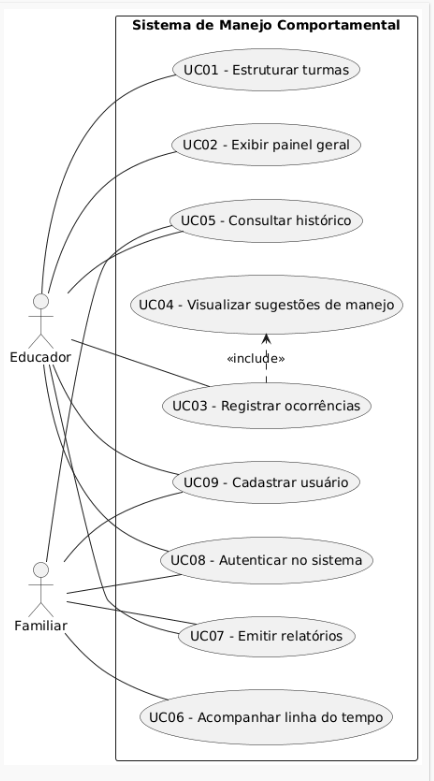
\includegraphics[width=0.3\textwidth, keepaspectratio]{dados/figuras/casoDeUso.png}
    
    \vspace{0.2cm}
    
    \begin{flushleft}
        \footnotesize Fonte: Elaborada pela autora (2026).
    \end{flushleft}
\end{figure}

Esses casos de uso reforçam o caráter pedagógico e de apoio clínico do sistema, oferecendo aos responsáveis um acompanhamento transparente e contínuo sobre a evolução comportamental do aluno. Dessa forma, a plataforma transcende a função de um simples diário escolar, atuando como uma ferramenta ativa que integra a família e a escola na aplicação de intervenções assertivas para o TDAH e o TOD.

\vspace{0.5cm}
\section{Protótipos}

Esta seção apresenta os protótipos de alta fidelidade desenvolvidos nas plataformas Figma \cite{figma2026} e Canva \cite{canva2026} para a aplicação web responsiva voltada ao suporte e manejo comportamental de alunos com TDAH e TOD. Os protótipos têm como objetivo representar o layout adaptável (para acesso em computadores institucionais e smartphones) e os principais elementos gráficos planejados para a implementação do sistema. A concepção das telas foi norteada por princípios de usabilidade e redução de carga cognitiva, adequando-se à realidade do público-alvo: professores com rotinas escolares aceleradas e familiares que buscam informações claras. Dessa forma, cada interface foi estruturada para oferecer uma navegação intuitiva, priorizando fluxos de registro ágeis, uma paleta de cores que transmite foco e acolhimento, e destaque visual imediato para as estratégias proativas de intervenção.

Para além do design, é fundamental compreender o fluxo operacional contínuo que rege a plataforma, estruturado para conectar as ações da escola ao acompanhamento da família. A jornada de uso inicia-se quando o educador acessa o sistema e visualiza o painel geral da sua turma, onde seleciona o perfil do aluno desejado. Diante de uma situação atípica, o professor registra a ocorrência de forma ágil. Imediatamente após o salvamento, o sistema processa o dado e exibe na tela cards com sugestões de manejo prático em tempo real. De forma simultânea, essa ação atualiza a linha do tempo (timeline) do estudante. Assim, a família pode acompanhar o histórico cronológico de eventos pelo celular, garantindo transparência e possibilitando a continuidade das abordagens terapêuticas no ambiente doméstico. A seguir, são detalhadas as telas que materializam esse fluxo.

\vspace{0.5cm}
\subsection{Tela de login}

A Figura 4.1 apresenta a tela inicial de autenticação (login) da plataforma. Nesta interface, o usuário é recebido por uma mensagem de boas-vindas e pelo lema "Educação com foco e cuidado". O destaque central da tela é a seleção do perfil de acesso, permitindo que o usuário identifique-se como “Educador” ou “Familiar” por meio de cartões amplos com ícones ilustrativos e intuitivos. Essa segregação inicial não é apenas visual, mas funcional: ela garante que o sistema direcione o educador para o painel de gestão da turma e o familiar para a linha do tempo do aluno, assegurando a privacidade dos dados de saúde e comportamento, conforme exigido pela LGPD.

Logo abaixo, encontram-se os campos minimalistas para a inserção das credenciais (e-mail e senha), atalhos para recuperação de acesso ou novo cadastro, e o botão principal ("Entrar"). O layout foi estruturado com base nos princípios de baixa carga cognitiva, utilizando cores suaves, amplo espaçamento em branco (white space) e áreas de toque facilitadas, garantindo uma navegação fluida tanto na versão desktop quanto na responsiva para dispositivos móveis.

\begin{figure}[H] 
    \centering
    \caption{Tela de login} % <-- Legenda ÚNICA no topo
    \label{fig:telas_login}
    \vspace{0.3cm}
    
    % --- Imagem A ---
    \begin{minipage}[b]{0.65\textwidth}
        \centering
        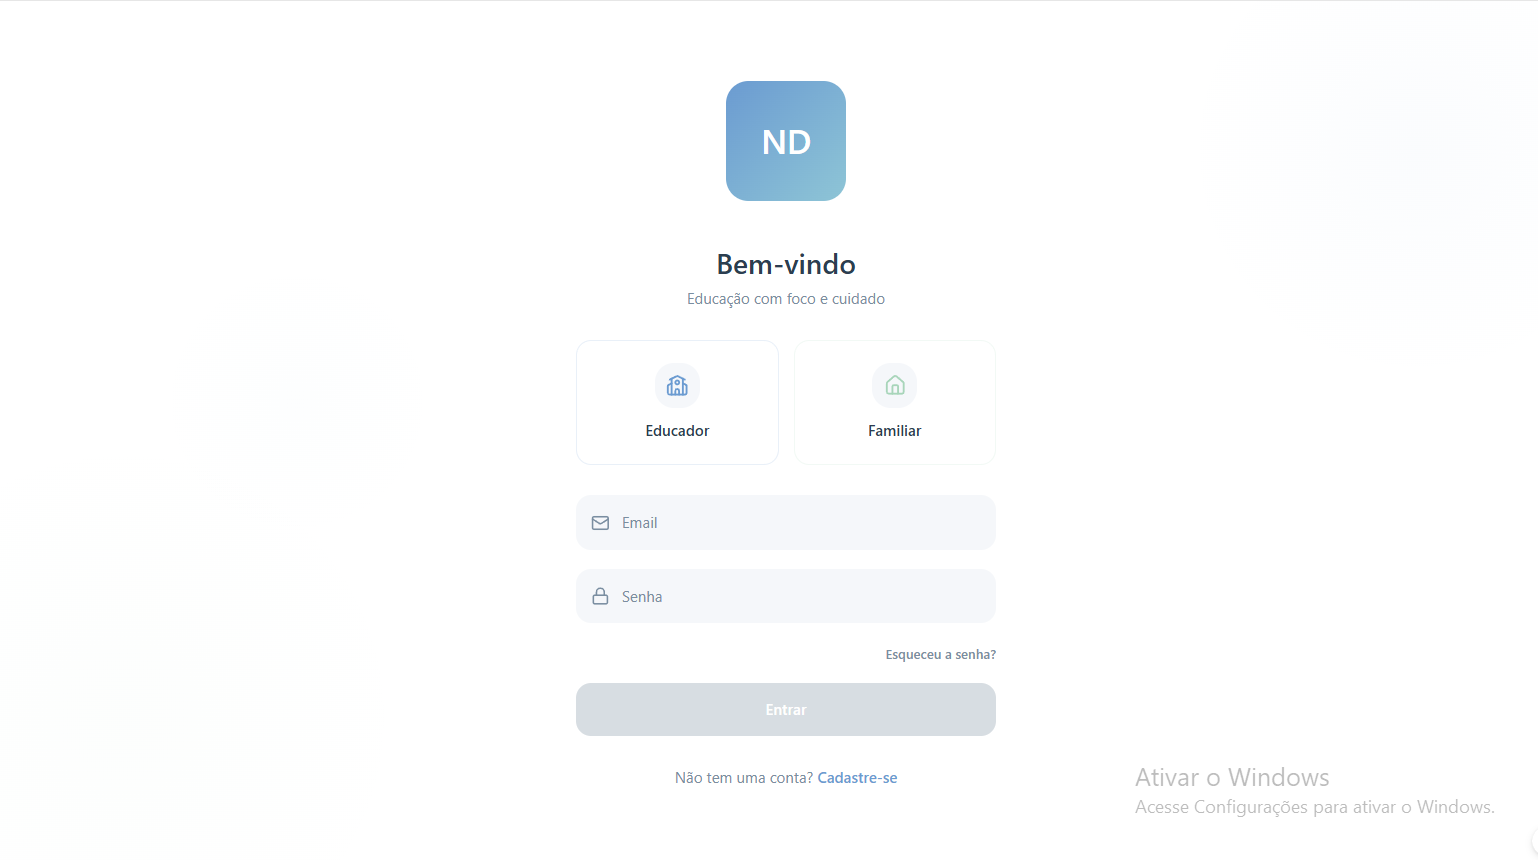
\includegraphics[height=9cm, keepaspectratio]{dados/figuras/telaLoginDesktop} 
        \centerline{\small (a) Desktop.} % <-- Subtítulo A
    \end{minipage}\hfill
    \rule{0.5pt}{10cm}\hfill % <-- 0.5pt é a espessura, 7cm é a altura
    % --- Imagem B ---
    \begin{minipage}[b]{0.30\textwidth}
        \centering
        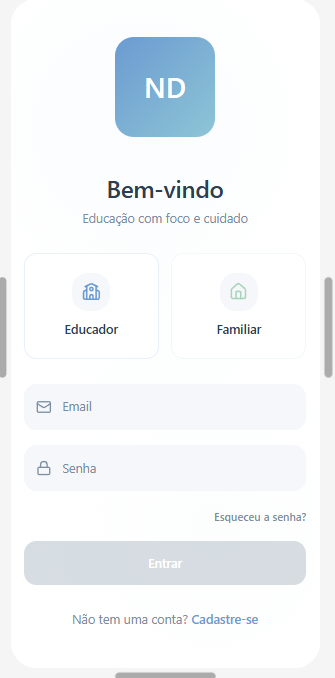
\includegraphics[height=9cm, keepaspectratio]{dados/figuras/telaLoginMobile}
        \centerline{\small (b) Mobile.} % <-- Subtítulo B
    \end{minipage}
    
   \vspace{0.3cm}
    \begin{flushleft} % <-- Inicia o alinhamento à esquerda
   \footnotesize{Fonte: Elaborada pela autora (2026).} % <-- Fonte ÚNICA no final
 \end{flushleft}   
\end{figure}

\vspace{0.5cm}
\subsection{Tela inicial para professor}

A Figura 4.2 apresenta o "Painel da Turma", a interface principal (dashboard) destinada ao perfil "Educador". O layout foi desenvolvido com foco primário na agilidade e na gestão visual, características essenciais para não sobrecarregar o docente durante a dinâmica da sala de aula. No topo da tela, destaca-se o botão de ação primária "+ Nova Ocorrência", dimensionado e posicionado estrategicamente para garantir o registro rápido de eventos comportamentais. 

    A listagem de alunos é apresentada por meio de cards minimalistas que incorporam indicadores visuais de status (pontos coloridos em tons suaves), permitindo ao professor monitorar o panorama da turma com uma leitura rápida e de baixo esforço cognitivo. Ademais, as telas evidenciam a arquitetura responsiva do sistema, demonstrando como a interface se adapta de forma fluida: operando em um formato de grade distribuída na visualização para computadores (desktop) e reorganizando-se automaticamente em uma lista vertical contínua na versão para dispositivos móveis (mobile), sem perda de funcionalidade ou usabilidade.

\begin{figure}[H] 
    \centering
    \caption{Tela inicial - professor} % <-- Legenda ÚNICA no topo
    \label{fig:telas_login}
    \vspace{0.3cm}
    
    % --- Imagem A ---
    \begin{minipage}[b]{0.65\textwidth}
        \centering
        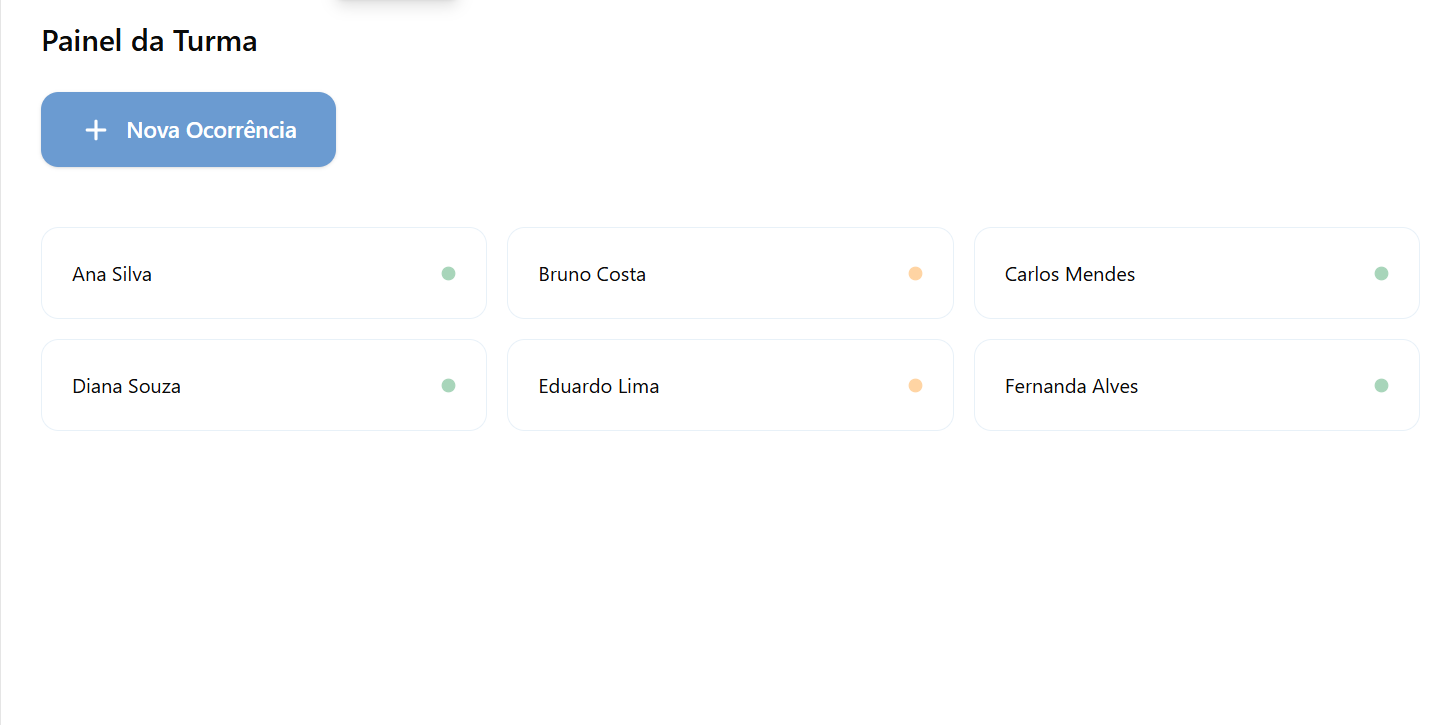
\includegraphics[height=9cm, keepaspectratio]{dados/figuras/telaInical_professorDesktop} 
        \centerline{\small (a) Desktop.} % <-- Subtítulo A
    \end{minipage}\hfill
    \rule{0.5pt}{10cm}\hfill % <-- 0.5pt é a espessura, 7cm é a altura
    % --- Imagem B ---
    \begin{minipage}[b]{0.30\textwidth}
        \centering
        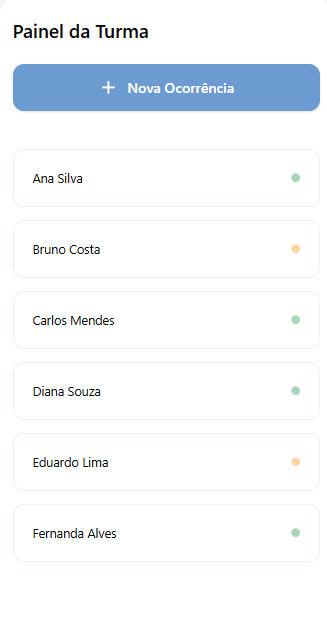
\includegraphics[height=9cm, keepaspectratio]{dados/figuras/telaInical_professorMobile}
        \centerline{\small (b) Mobile.} % <-- Subtítulo B
    \end{minipage}
    
   \vspace{0.3cm}
    \begin{flushleft} % <-- Inicia o alinhamento à esquerda
   \footnotesize{Fonte: Elaborada pela autora (2026).} % <-- Fonte ÚNICA no final
 \end{flushleft}   
\end{figure}

\vspace{0.5cm}
\subsection{Tela inicial para os familiares}

A Figura 4.3 ilustra a interface principal destinada ao perfil "Familiar", apresentada nas suas versões desktop e mobile. Em oposição a um painel de controlo complexo, esa tela adota o formato de uma linha do tempo (timeline) cronológica, assemelhando-se a um feed de atualizações. No topo, a identificação clara do aluno estabelece imediatamente o contexto de navegação. O corpo da interface exibe os registros diários — tais como comportamentos positivos, ocorrências de agitação e avisos pedagógicos — através de cards informativos, acompanhados da respetiva hora de registo. 

A utilização de ícones intuitivos e de uma paleta de cores funcional e suave (como o verde para atitudes colaborativas e o azul para alertas e ocorrências) permite uma compreensão visual imediata. A arquitetura responsiva garante que os familiares possam aceder à rotina escolar com clareza, tanto em computadores como em telefones, promovendo uma comunicação transparente e ágil entre a escola e a família, sempre a respeitar o princípio de baixa carga cognitiva.

\begin{figure}[H] 
    \centering
    \caption{Tela inicial - familiares} % <-- Legenda ÚNICA no topo
    \label{fig:telas_login}
    \vspace{0.3cm}
    
    % --- Imagem A ---
    \begin{minipage}[b]{0.65\textwidth}
        \centering
        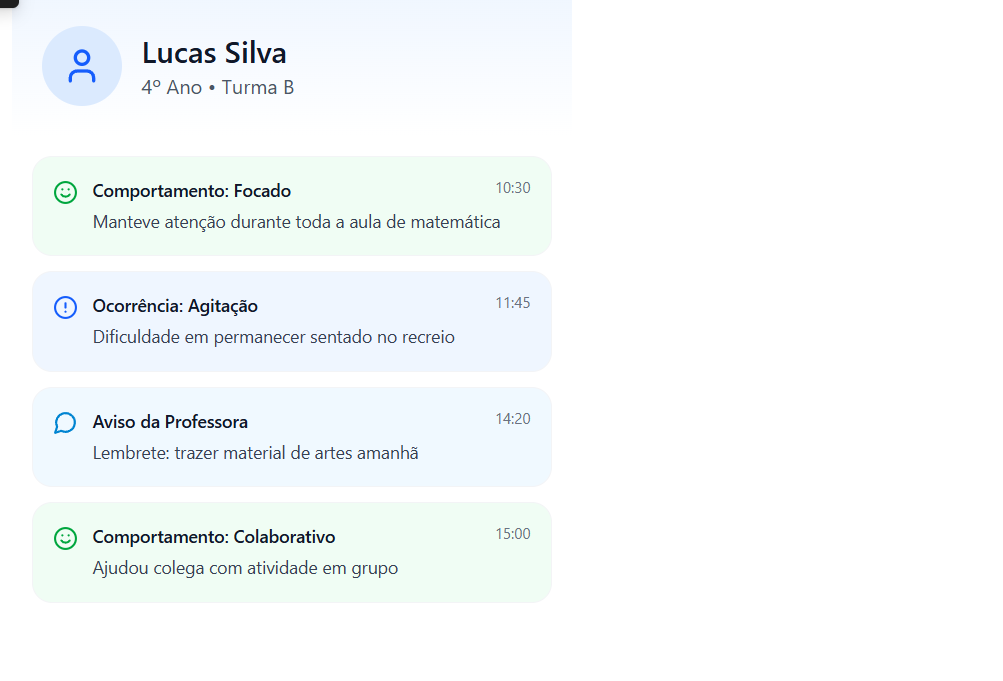
\includegraphics[height=9cm, keepaspectratio]{dados/figuras/telaInical_familiarDesktop} 
        \centerline{\small (a) Desktop.} % <-- Subtítulo A
    \end{minipage}\hfill
    \rule{0.5pt}{10cm}\hfill % <-- 0.5pt é a espessura, 7cm é a altura
    % --- Imagem B ---
    \begin{minipage}[b]{0.30\textwidth}
        \centering
        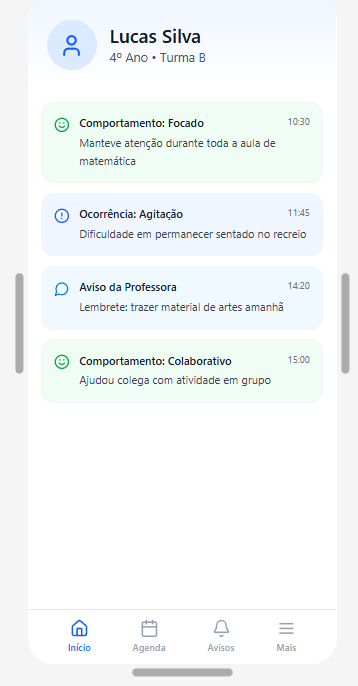
\includegraphics[height=9cm, keepaspectratio]{dados/figuras/telaInical_familiarMobile}
        \centerline{\small (b) Mobile.} % <-- Subtítulo B
    \end{minipage}
    
   \vspace{0.3cm}
    \begin{flushleft} % <-- Inicia o alinhamento à esquerda
   \footnotesize{Fonte: Elaborada pela autora (2026).} % <-- Fonte ÚNICA no final
 \end{flushleft}   
\end{figure}

\vspace{0.5cm}
\subsection{Tela de registro de ocorrências}

A Figura 4.4 ilustra o ecrã de novo registo de ocorrências, desenvolvido em exclusivo para o perfil de educador, apresentado nas suas vertentes mobile e desktop. O design desta interface foi concebido com foco absoluto na agilidade e na otimização do tempo, uma exigência crítica para não interromper a dinâmica da sala de aula. Para tal, minimizou-se a dependência de campos de texto livre, substituindo-os por botões de seleção rápida (chips ou tags) que categorizam os comportamentos típicos do TDAH e TOD (como agitação, desatenção e impulsividade) e os seus respectivos níveis de intensidade. 

O campo para observações textuais foi mantido estritamente como opcional. Esta abordagem não só padroniza a recolha de dados, como também reduz drasticamente a carga cognitiva exigida ao professor no momento de uma crise. Por fim, o botão de ação primária ("Salvar e Ver Sugestões") evidencia o grande diferencial do sistema: a transição imediata do registo passivo para o suporte pedagógico proativo.

\begin{figure}[H] 
    \centering
    \caption{Tela de registro de ocorrências} % <-- Legenda ÚNICA no topo
    \label{fig:telas_login}
    \vspace{0.3cm}
    
    % --- Imagem A ---
    \begin{minipage}[b]{0.65\textwidth}
        \centering
        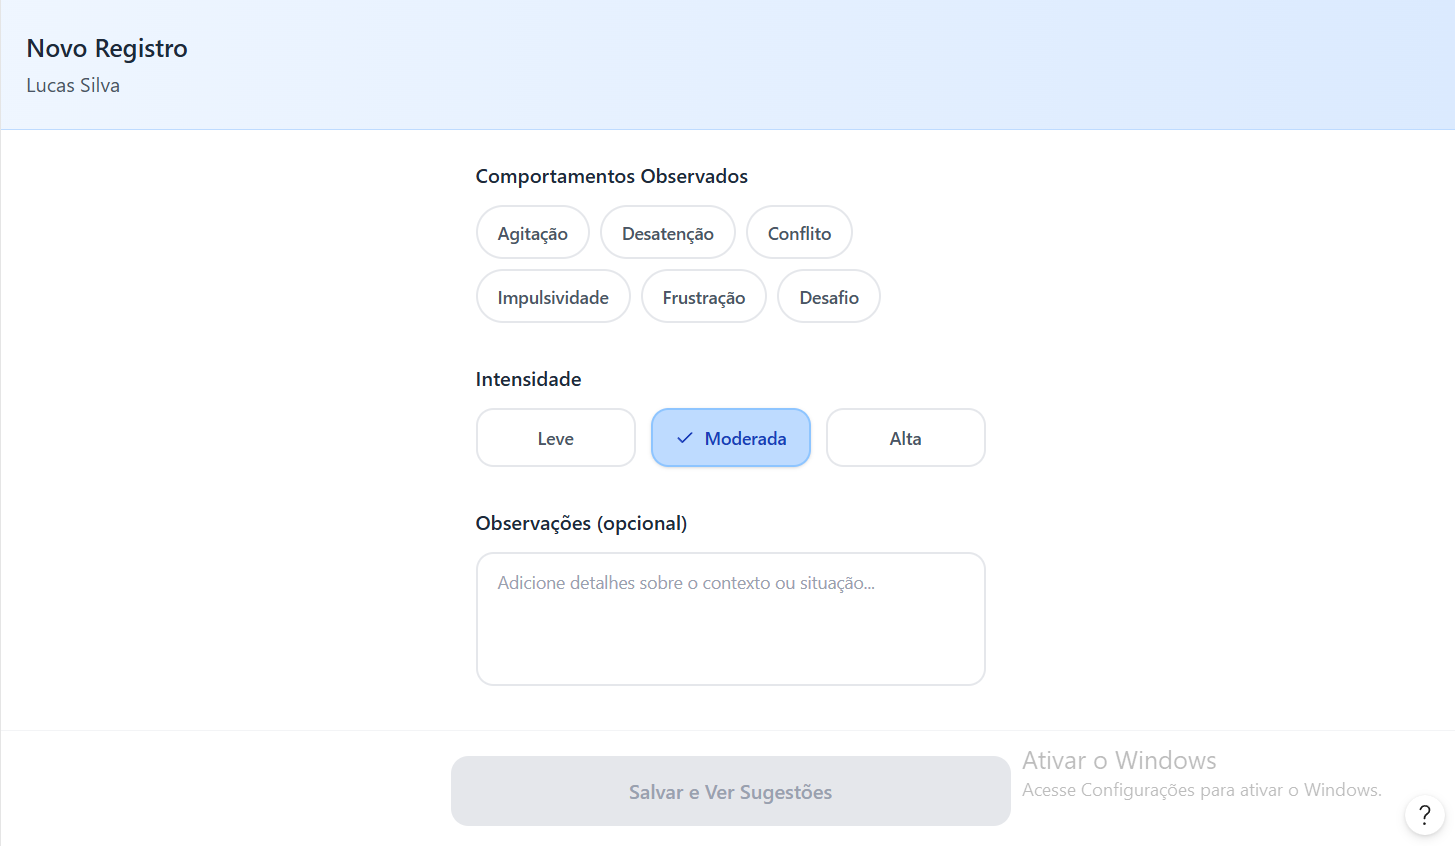
\includegraphics[height=9cm, keepaspectratio]{dados/figuras/ocorrenciasDesktop} 
        \centerline{\small (a) Desktop.} % <-- Subtítulo A
    \end{minipage}\hfill
    \rule{0.5pt}{10cm}\hfill % <-- 0.5pt é a espessura, 7cm é a altura
    % --- Imagem B ---
    \begin{minipage}[b]{0.30\textwidth}
        \centering
        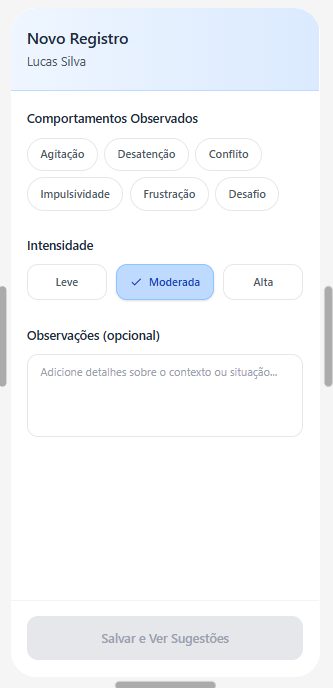
\includegraphics[height=9cm, keepaspectratio]{dados/figuras/ocorrenciasMobile}
        \centerline{\small (b) Mobile.} % <-- Subtítulo B
    \end{minipage}
    
   \vspace{0.3cm}
    \begin{flushleft} % <-- Inicia o alinhamento à esquerda
   \footnotesize{Fonte: Elaborada pela autora (2026).} % <-- Fonte ÚNICA no final
 \end{flushleft}   
\end{figure}

\vspace{0.5cm}
\subsection{Tela de estratégias de manejo}

A Figura 4.5 apresenta a interface de Estratégias de Manejo, que constitui o principal diferencial pedagógico e tecnológico da plataforma. Ao concluir o registro de uma ocorrência, o educador é imediatamente direcionado para esta tela, que atua como um assistente proativo. Em vez de apenas armazenar passivamente o dado comportamental, o sistema filtra e exibe cards com sugestões de intervenção baseadas em evidências para o TDAH e TOD, contextualizadas com o comportamento recém-registrado (como, por exemplo, pausas para movimento ou reforço positivo imediato). 

O design da interface mantém a coerência visual das telas anteriores, priorizando o baixo peso cognitivo: as instruções são curtas, objetivas e acompanhadas de ícones claros, garantindo que o professor possa ler e aplicar a estratégia em questão de segundos, promovendo a autorregulação do aluno e a minimização de conflitos no ambiente escolar.

\begin{figure}[H] 
    \centering
    \caption{Tela de registro de ocorrências} % <-- Legenda ÚNICA no topo
    \label{fig:telas_login}
    \vspace{0.3cm}
    
    % --- Imagem A ---
    \begin{minipage}[b]{0.65\textwidth}
        \centering
        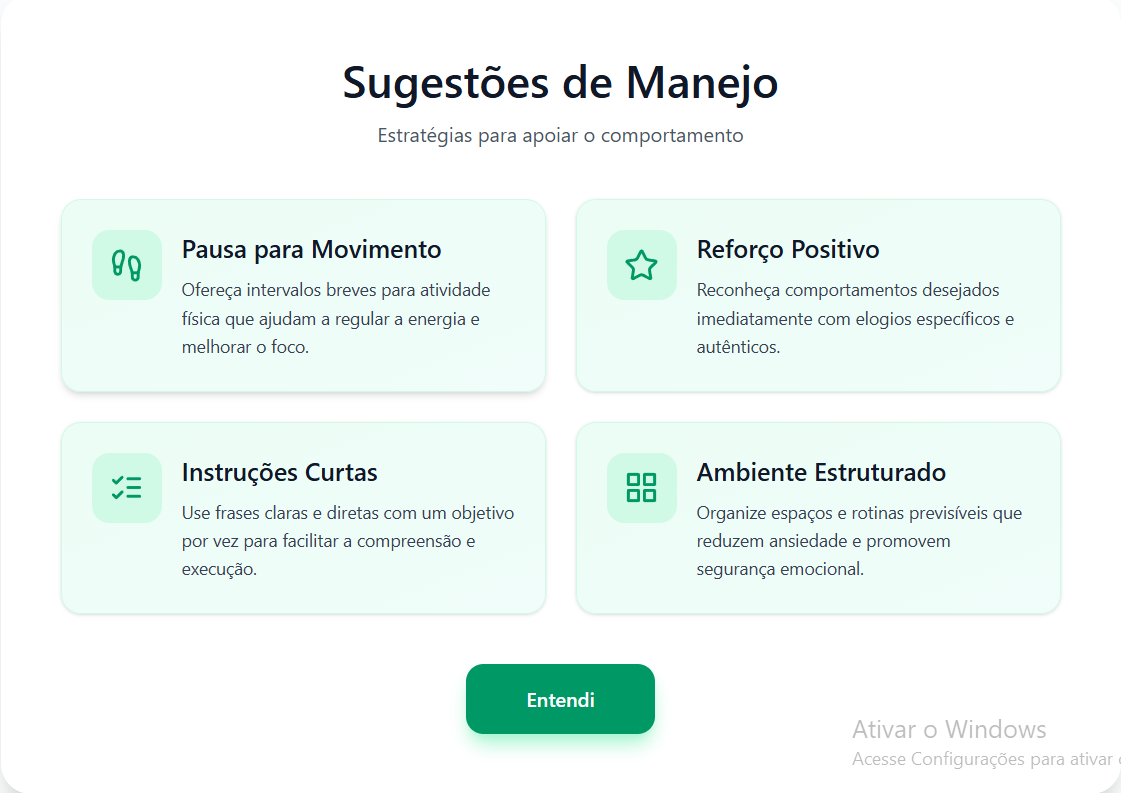
\includegraphics[height=9cm, keepaspectratio]{dados/figuras/estrategiaDeManejo_desktop} 
        \centerline{\small (a) Desktop.} % <-- Subtítulo A
    \end{minipage}\hfill
    \rule{0.5pt}{10cm}\hfill % <-- 0.5pt é a espessura, 7cm é a altura
    % --- Imagem B ---
    \begin{minipage}[b]{0.30\textwidth}
        \centering
        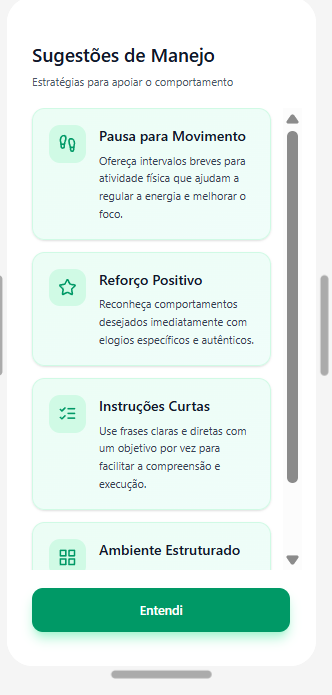
\includegraphics[height=9cm, keepaspectratio]{dados/figuras/estrategiaDeManejo_mobile}
        \centerline{\small (b) Mobile.} % <-- Subtítulo B
    \end{minipage}
    
   \vspace{0.3cm}
    \begin{flushleft} % <-- Inicia o alinhamento à esquerda
   \footnotesize{Fonte: Elaborada pela autora (2026).} % <-- Fonte ÚNICA no final
 \end{flushleft}   
\end{figure}

\vspace{0.5cm}
\subsection{Tela da linha do tempo da família}

A Figura 4.6 apresenta a tela de histórico diário do aluno, estruturada em formato de linha do tempo (timeline), em suas versões mobile e desktop. Esta interface funciona como o principal canal de acompanhamento para a família e como registro de consulta para o educador. O layout reforça a premissa de baixa carga cognitiva ao destacar, no topo, a identificação clara do estudante. O fluxo central é composto por cards de eventos organizados cronologicamente, que empregam uma categorização visual baseada em cores e ícones específicos: verde para comportamentos positivos e foco, azul para avisos ou comunicações neutras, e laranja para alertas comportamentais de agitação. 

Essa sinalização visual permite aos usuários uma assimilação imediata do estado do aluno, sem a necessidade de uma leitura exaustiva. Adicionalmente, as imagens evidenciam a arquitetura responsiva do sistema, ilustrando a adaptação da barra de navegação — posicionada no rodapé nos celulares e na lateral esquerda nos computadores — de modo a preservar a ergonomia e a acessibilidade em qualquer dispositivo.

\begin{figure}[H] 
    \centering
    \caption{Tela da linha do tempo da família} % <-- Legenda ÚNICA no topo
    \label{fig:telas_login}
    \vspace{0.3cm}
    
    % --- Imagem A ---
    \begin{minipage}[b]{0.65\textwidth}
        \centering
        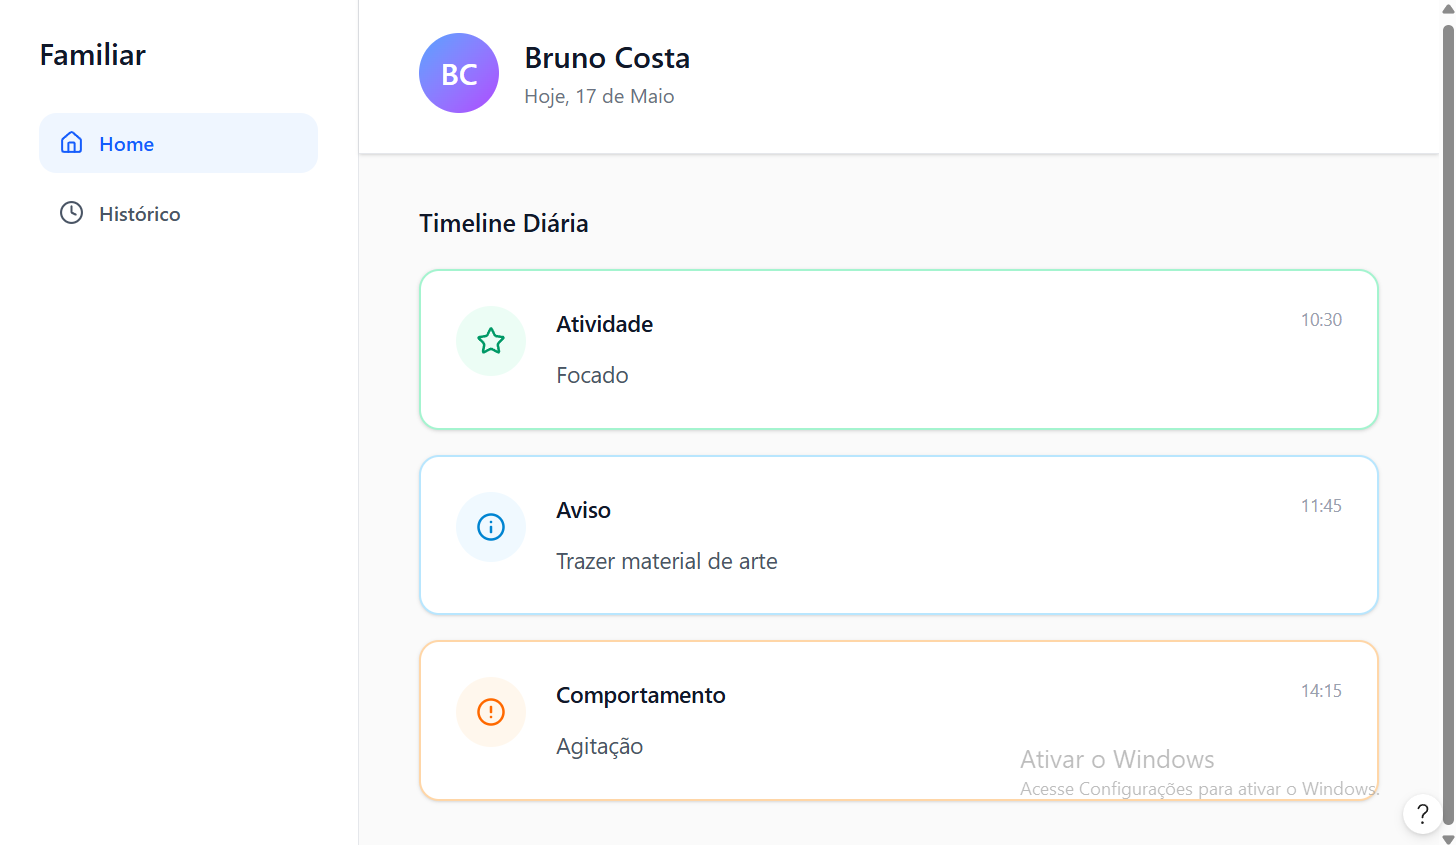
\includegraphics[height=9cm, keepaspectratio]{dados/figuras/timeline_Desktop} 
        \centerline{\small (a) Desktop.} % <-- Subtítulo A
    \end{minipage}\hfill
    \rule{0.5pt}{10cm}\hfill % <-- 0.5pt é a espessura, 7cm é a altura
    % --- Imagem B ---
    \begin{minipage}[b]{0.30\textwidth}
        \centering
        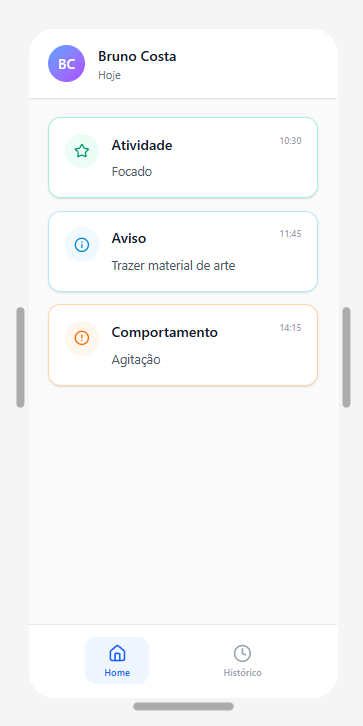
\includegraphics[height=9cm, keepaspectratio]{dados/figuras/timelineMobile}
        \centerline{\small (b) Mobile.} % <-- Subtítulo B
    \end{minipage}
    
   \vspace{0.3cm}
    \begin{flushleft} % <-- Inicia o alinhamento à esquerda
   \footnotesize{Fonte: Elaborada pela autora (2026).} % <-- Fonte ÚNICA no final
 \end{flushleft}   
\end{figure}